Idea: Project $x$ on $w$, which gets us the large vector from the origin to the tip of the dotted line in figure~\ref{fig:sketch}}. From this we have to subtract the length of the part from the origin to the decision boundary, which will be  $\alpha$.
\begin{figure}[h]
	\centering
	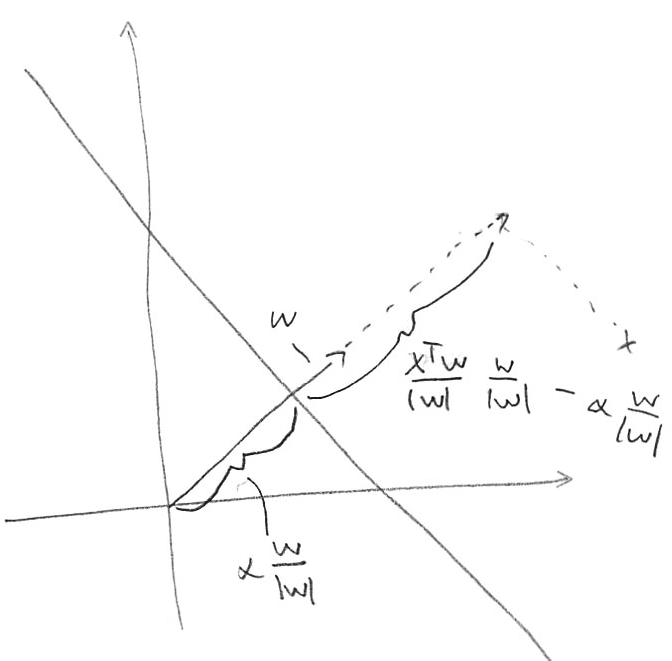
\includegraphics[width=0.5\textwidth]{sketch}
	\caption{sketch for 8.3b}
	\label{fig:sketch}
\end{figure}

Let $x$ be any closest point.
The projection of $x$ onto $w$ is is $\frac{x^Tw}{|w|} \frac{w}{|w|}$, where $\frac{w}{|w|}$ is a unit vector.

Calculate $\alpha$ (the scalar to stretch $\frac{w}{|w|}$ by to reach the boundary):
\begin{align*}
	& w^T(\alpha \frac{w}{|w|}) + b = 0 \\
	\Leftrightarrow\ & \frac{\alpha}{|w|}w^T(w) + b = 0 \\
	\Leftrightarrow\ & \frac{\alpha}{|w|}\underbrace{w^Tw}_{|w|^2} + b = 0 \\
	\Leftrightarrow\ & \frac{\alpha}{|w|}|w|^2 + b = 0 \\
	\Leftrightarrow\ & \alpha|w| + b = 0 \\
	\Leftrightarrow\ & \alpha = \frac{-b}{|w|}
\end{align*}

Then the distance of $x$ to the decision boundary is:
\begin{align*}
	d=\ & \left\Vert\frac{x^Tw}{|w|} \frac{w}{|w|}\right\Vert - \left\Vert\alpha \frac{w}{|w|}\right\Vert \\
	=\ & \frac{x^Tw}{|w|} - \frac{-b}{|w|} \\
	=\ & \frac{x^Tw + b}{|w|} \qquad\left\vert \text{for the closest point: } w^Tx + b = 1\\
	=\ & \frac{1}{|w|} \\
\end{align*}

For points farther away than $x$ the term $\frac{x^Tw}{|w|} \frac{w}{|w|}$ increases, while $\alpha \frac{w}{|w|}$ stays the same. Hence the distance gets larger, so overall: $d \geq \frac{1}{|w|}$
